\section{Analisi Comparativa}

\subsection{Introduzione}
Il presente documento si pone l'obiettivo di evolvere lo studio di mercato già avviato nelle fasi preliminari del progetto Culturia~\cite{culturia_repo}. Sebbene l'analisi originaria si focalizzasse principalmente sulla dimensione social e sulla digitalizzazione dei beni culturali, la nuova direzione progettuale richiede una rilettura critica del panorama tecnologico, ponendo al centro la \textbf{Realtà Aumentata (AR)} e l'\textbf{Inclusività} (accessibilità sensoriale, motoria e cognitiva).

Per condurre questa analisi, abbiamo individuato tre sistemi emblematici:
\begin{itemize}
    \item \textbf{Google Arts \& Culture:} Focalizzato su esposizioni immersive e modelli 3D ad alta fedeltà.
    \item \textbf{Smartify:} Utilizza la \textit{Computer Vision} per fornire audioguide e contenuti interattivi on-site.
    \item \textbf{Lazarillo:} Focalizzato sull'orientamento per persone con disabilità visive tramite feedback audio.
\end{itemize}

\subsection{Analisi dei competitor}
Prima di procedere alla valutazione comparativa, è essenziale delineare il profilo funzionale dei sistemi selezionati, evidenziando la loro filosofia progettuale e il loro raggio d'azione.

\paragraph{Google Arts \& Culture} È la piattaforma leader per la digitalizzazione globale del patrimonio culturale. Attraverso tecnologie di acquisizione ad altissima risoluzione e tour virtuali a 360°, permette di esplorare migliaia di musei e siti storici. Tuttavia, la sua natura di "archivio universale" la rende più adatta a una fruizione remota e contemplativa che a un'assistenza dinamica on-site.

\paragraph{Smartify} Definita spesso lo "Shazam per l'arte", l'applicazione utilizza il riconoscimento visivo per identificare istantaneamente le opere, fornendo audioguide e approfondimenti curati. Sebbene sia estremamente efficace nei grandi poli museali partner, soffre di un database limitato che tende a escludere i siti minori e i contesti periferici.

\paragraph{Lazarillo} Rappresenta uno strumento di navigazione pura progettato per persone con disabilità visive. Grazie a feedback audio in tempo reale, guida l'utente nello spazio fisico. Essendo un sistema puramente funzionale, non integra alcuna narrazione culturale, limitandosi a mappare la geometria e i servizi dell'ambiente.

\newpage
\subsubsection{Studio comparativo e impatto sulle Personas}
Nella seguente tabella vengono sintetizzati i punti di forza e le aree di criticità dei competitor, rapportandoli alle esigenze specifiche delle nostre \textit{Personas}.

\vspace{-0.2cm}
\begin{table}[H]
    \centering
    \caption{Analisi comparativa dei competitor rispetto ai task e alle Personas.}
    \vspace{0.15cm}
    \small
    \tabcolsep=3pt
    \renewcommand{\arraystretch}{1.4}
    \begin{tabularx}{\textwidth}{@{} c m{2.2cm} X X X @{}}
        \toprule
        \textbf{Logo} & \textbf{Sistema} & \textbf{Punti di Forza} & \textbf{Punti di Debolezza} & \textbf{Persona Impact} \\
        \midrule
        \raisebox{-0.4\height}{
\includegraphics[width=1.5cm]{img/google_arts_and_culture_logo.png}} & 
        \textbf{Google Arts \& Culture} & 
        Eccellenza visiva 3D; accesso remoto universale e gratuito. & 
        Fruizione passiva; scarsa utilità nell'orientamento fisico reale. & 
        Soddisfa \textbf{Elena} (dettagli), ma non guida \textbf{Matteo}. \\ \addlinespace
        
        \raisebox{-0.4\height}{
\includegraphics[width=1.5cm]{img/Smartify_Logo.png}} & 
        \textbf{Smartify} & 
        Riconoscimento rapido dell'opera; audioguide professionali. & 
        Database limitato; non supporta piccoli borghi. & 
        Ideale per gli highlights rapidi di \textbf{Marco}. \\ \addlinespace
        
        \raisebox{-0.4\height}{
\includegraphics[width=1.5cm]{img/Lazarillo_logo.png}} & 
        \textbf{Lazarillo} & 
        Precisione assoluta per l'accessibilità sensoriale e motoria. & 
        Interfaccia funzionale; assenza di narrazione culturale. & 
        Supporta \textbf{Giovanni} nell'assistenza inclusiva. \\
        \bottomrule
    \end{tabularx}
\end{table}

\subsection{Carenze dei sistemi analizzati}
Sebbene i sistemi presentino tecnologie avanzate, l'analisi ha evidenziato diverse carenze strutturali che Culturia mira a colmare:
\begin{itemize}
    \item \textbf{Google Arts \& Culture:} Il limite principale è l'impossibilità di una reale integrazione on-site; il sistema è concepito per la fruizione virtuale da remoto, mancando di strumenti che supportino il visitatore una volta giunto fisicamente sul luogo culturale.
    \item \textbf{Smartify:} Il sistema di riconoscimento basato su database commerciali non è scalabile per i piccoli borghi. La mancanza di documentazione per le opere minori rende l'app quasi inutilizzabile in contesti periferici o siti archeologici meno noti, lasciando un vuoto comunicativo proprio dove il bisogno di valorizzazione è maggiore.
    \item \textbf{Lazarillo:} L'interfaccia si presenta estremamente spartana e specialistica, essendo progettata quasi esclusivamente per non vedenti. Manca di supporto per altre tipologie di disabilità (cognitive o uditive) e non offre una contestualizzazione culturale specifica, limitandosi a funzioni di navigazione pura.
\end{itemize}

\subsection{Posizionamento Strategico e Gap Analysis}
Il posizionamento di Culturia si distingue per la capacità di coniugare un'alta \textit{Inclusività Multimodale} con la \textit{Fattibilità per i Piccoli Borghi}. A differenza dei grandi player o degli strumenti specialistici, Culturia si pone come un \textbf{Hub Unificato}.

Il valore differenziante di Culturia emerge con chiarezza dal confronto con i limiti dei sistemi analizzati. Mentre i grandi player si concentrano sulla conservazione digitale "distante" o su audioguide per musei di fama mondiale, Culturia abilita la \textbf{valorizzazione on-site del micro-patrimonio}.

A differenza di \textbf{Google Arts \& Culture}, il nostro sistema non è una finestra virtuale ma uno strumento di esplorazione dinamica sul campo, che accompagna il visitatore nella scoperta della realtà che lo circonda. Rispetto a \textbf{Smartify}, Culturia abbatte la barriera della "notorietà": tramite l'\textit{Hub Unificato}, anche le amministrazioni dei piccoli borghi possono digitalizzare e rendere fruibile il proprio patrimonio senza dipendere da database proprietari o investimenti insostenibili, democratizzando l'accesso alla visibilità turistica.

Infine, superando l'approccio puramente funzionale di \textbf{Lazarillo}, Culturia propone un'accessibilità che non sacrifica il piacere estetico e narrativo. L'integrazione tra \textbf{AR Spaziale} e il \textbf{Cicerone IA} trasforma la navigazione in un racconto inclusivo e multimodale, dove l'informazione è sintetizzata per adattarsi alle diverse abilità del visitatore, garantendo che nessuno sia escluso dall'emozione della scoperta culturale. Questo approccio risponde direttamente ai task dell'Assignment 1, trasformando siti minori in esperienze immersive, accessibili e tecnologicamente democratiche.

\begin{figure}[H]
    \centering
    \begin{tikzpicture}
        % ── Griglia sottile ──
        \draw[gray!20, very thin] (0,0) grid[step=1] (10,10);

        % ── Linee mediane tratteggiate ──
        \draw[gray!35, dashed, thin] (5,0) -- (5,10);
        \draw[gray!35, dashed, thin] (0,5) -- (10,5);

        % ── Assi principali ──
        \draw[culturiaRed, very thick, -stealth] (-0.3,0) -- (10.8,0);
        \draw[culturiaRed, very thick, -stealth] (0,-0.3) -- (0,10.8);

        % ── Label assi ──
        \node[culturiaRed, font=\sffamily\bfseries\footnotesize, anchor=north] at (5,-0.6) {Fattibilità per i Piccoli Borghi};
        \node[culturiaRed, font=\sffamily\bfseries\footnotesize, anchor=south, rotate=90] at (-0.6,5) {Inclusività Multimodale};

        % ── Competitor: Google Arts & Culture (abbassato) ──
        \node[inner sep=0pt] (google) at (2,4) {
\includegraphics[width=1cm]{img/google_arts_and_culture_logo.png}};
        \node[font=\sffamily\tiny, anchor=north] at (google.south) {Google A\&C};

        % ── Competitor: Smartify (più a sinistra) ──
        \node[inner sep=0pt] (smartify) at (2.5,5.5) {
\includegraphics[width=1cm]{img/Smartify_Logo.png}};
        \node[font=\sffamily\tiny, anchor=north] at (smartify.south) {Smartify};

        % ── Competitor: Lazarillo (al centro) ──
        \node[inner sep=0pt] (lazarillo) at (5,5) {
\includegraphics[width=1cm]{img/Lazarillo_logo.png}};
        \node[font=\sffamily\tiny, anchor=north] at (lazarillo.south) {Lazarillo};

        % ── Culturia: quadrante premium in alto a destra ──
        \node[inner sep=0pt] (culturia) at (8.8,9) {
\includegraphics[width=1.2cm]{img/LogoCulturia.png}};
        \node[culturiaRed, font=\sffamily\bfseries\small, anchor=south] at (culturia.north) {Culturia};

    \end{tikzpicture}
    \caption{Matrice di posizionamento: Inclusività vs Fattibilità per i Piccoli Borghi.}
\end{figure}

\newpage
\subsection{Acquisizione Media: Screenshots dei sistemi}
In questa sezione vengono presentati gli screenshot acquisiti dai sistemi analizzati, raggruppati per applicazione, per evidenziare le diverse logiche di interfaccia e funzionalità.

\subsubsection{Google Arts \& Culture}
L'app si distingue per l'alta qualità delle immagini e la natura immersiva dei tour virtuali, ma evidenzia la sua natura prettamente "remota".
\nopagebreak
\begin{figure}[H]
    \centering
    \begin{minipage}{0.31\textwidth}
        \centering
        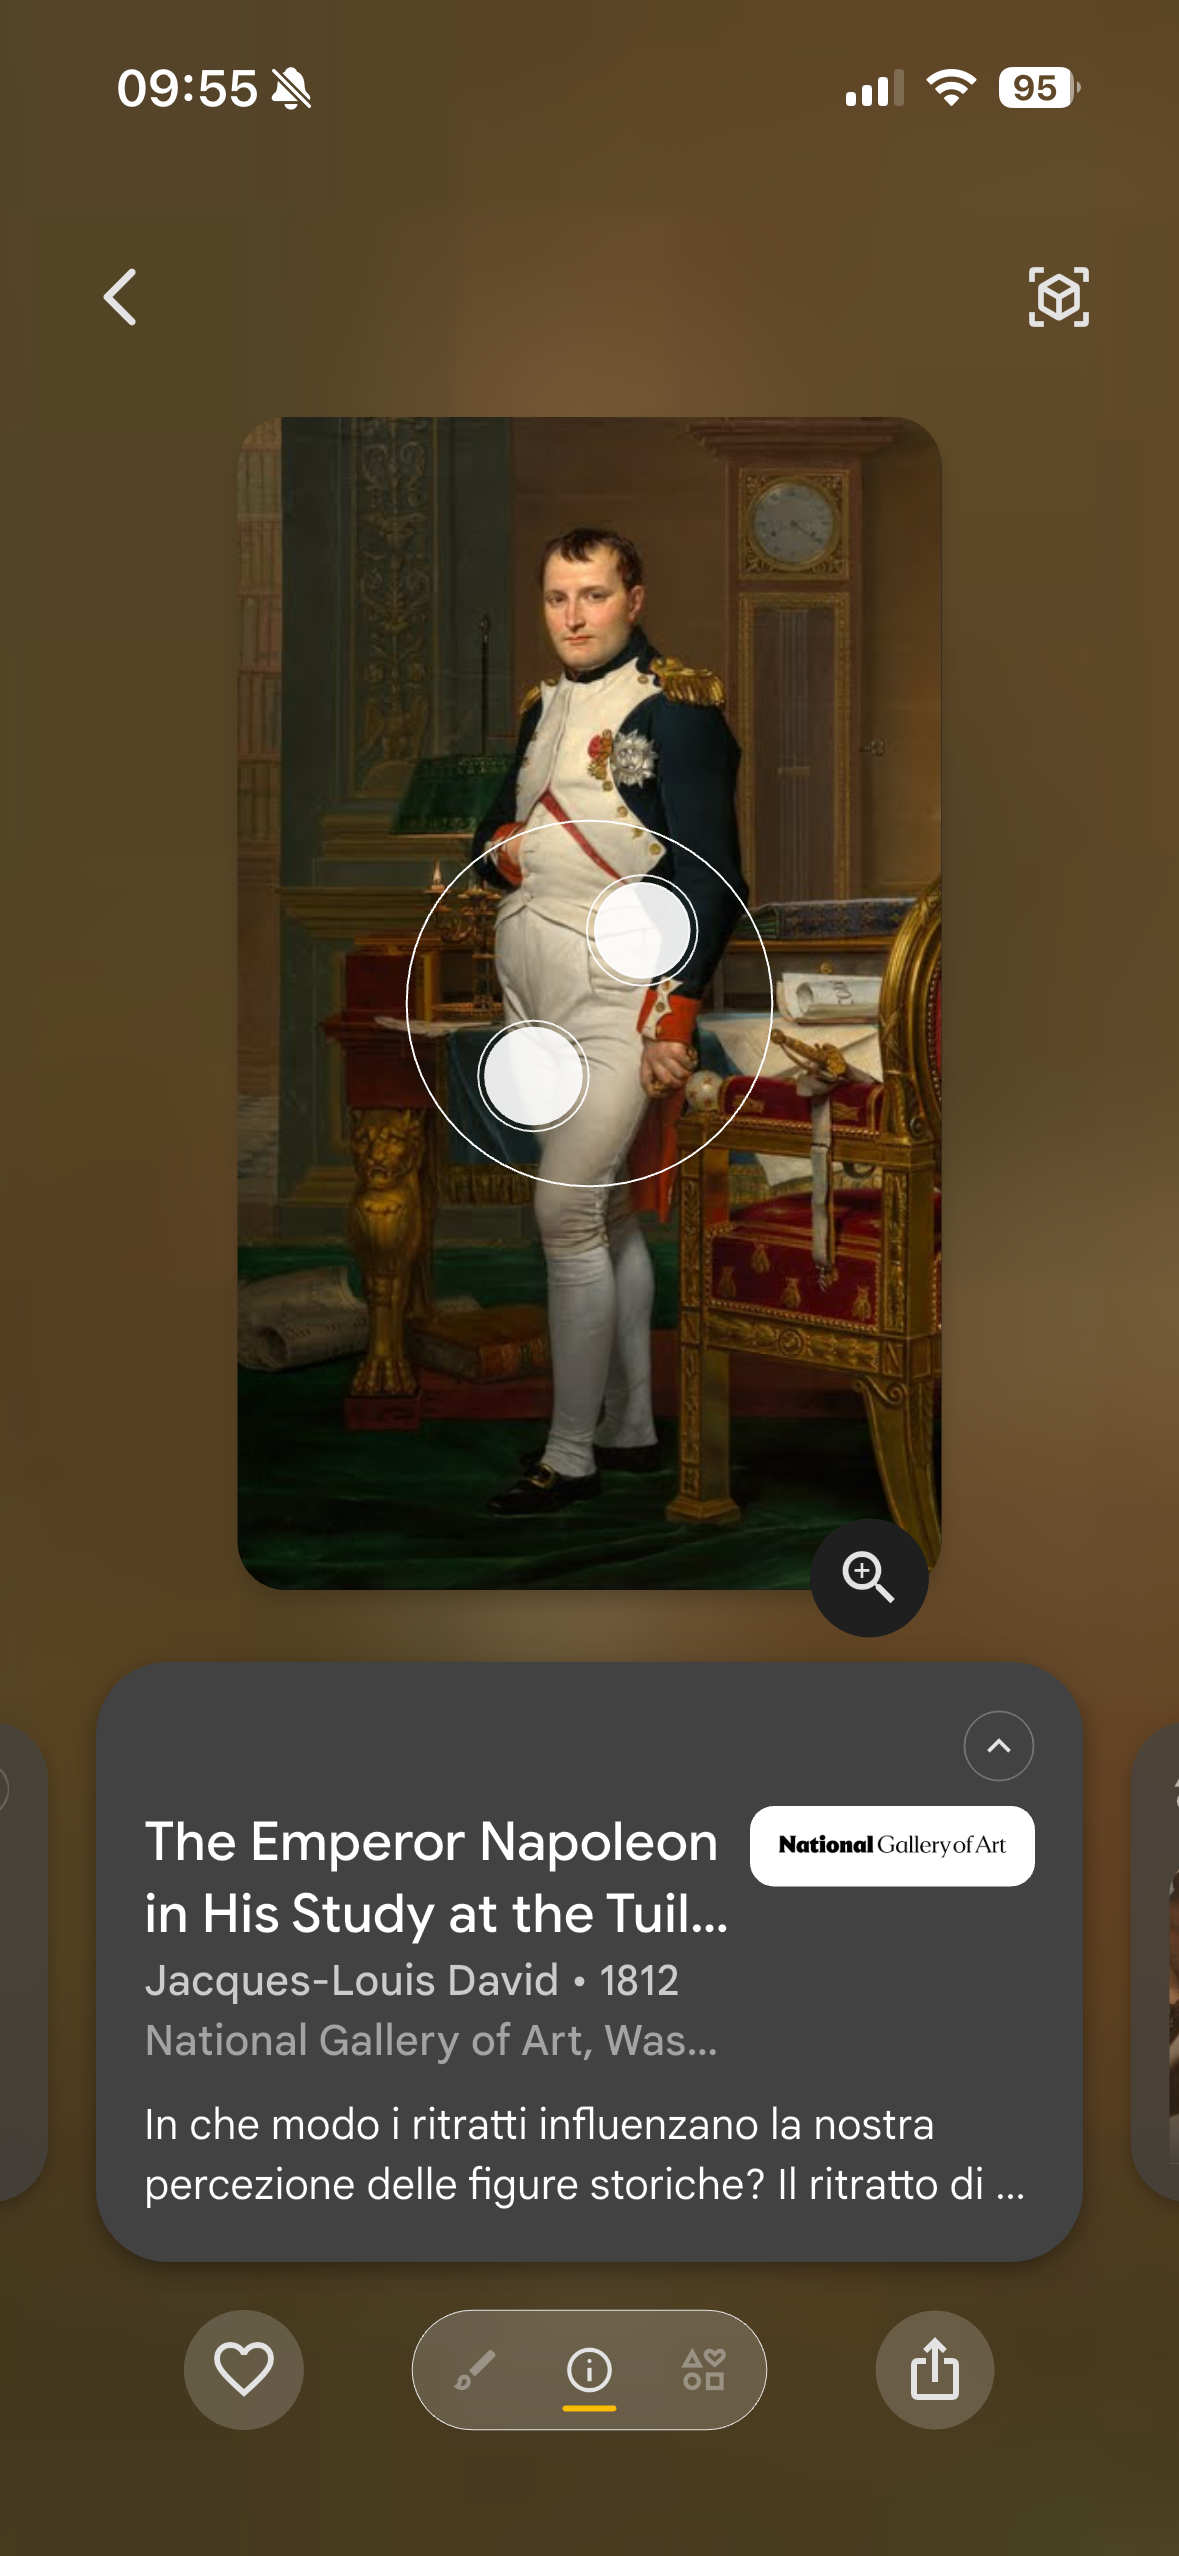
\includegraphics[width=\textwidth]{img/GA&C_01.PNG}
        \caption*{Pocket Gallery}
    \end{minipage}
    \hfill
    \begin{minipage}{0.31\textwidth}
        \centering
        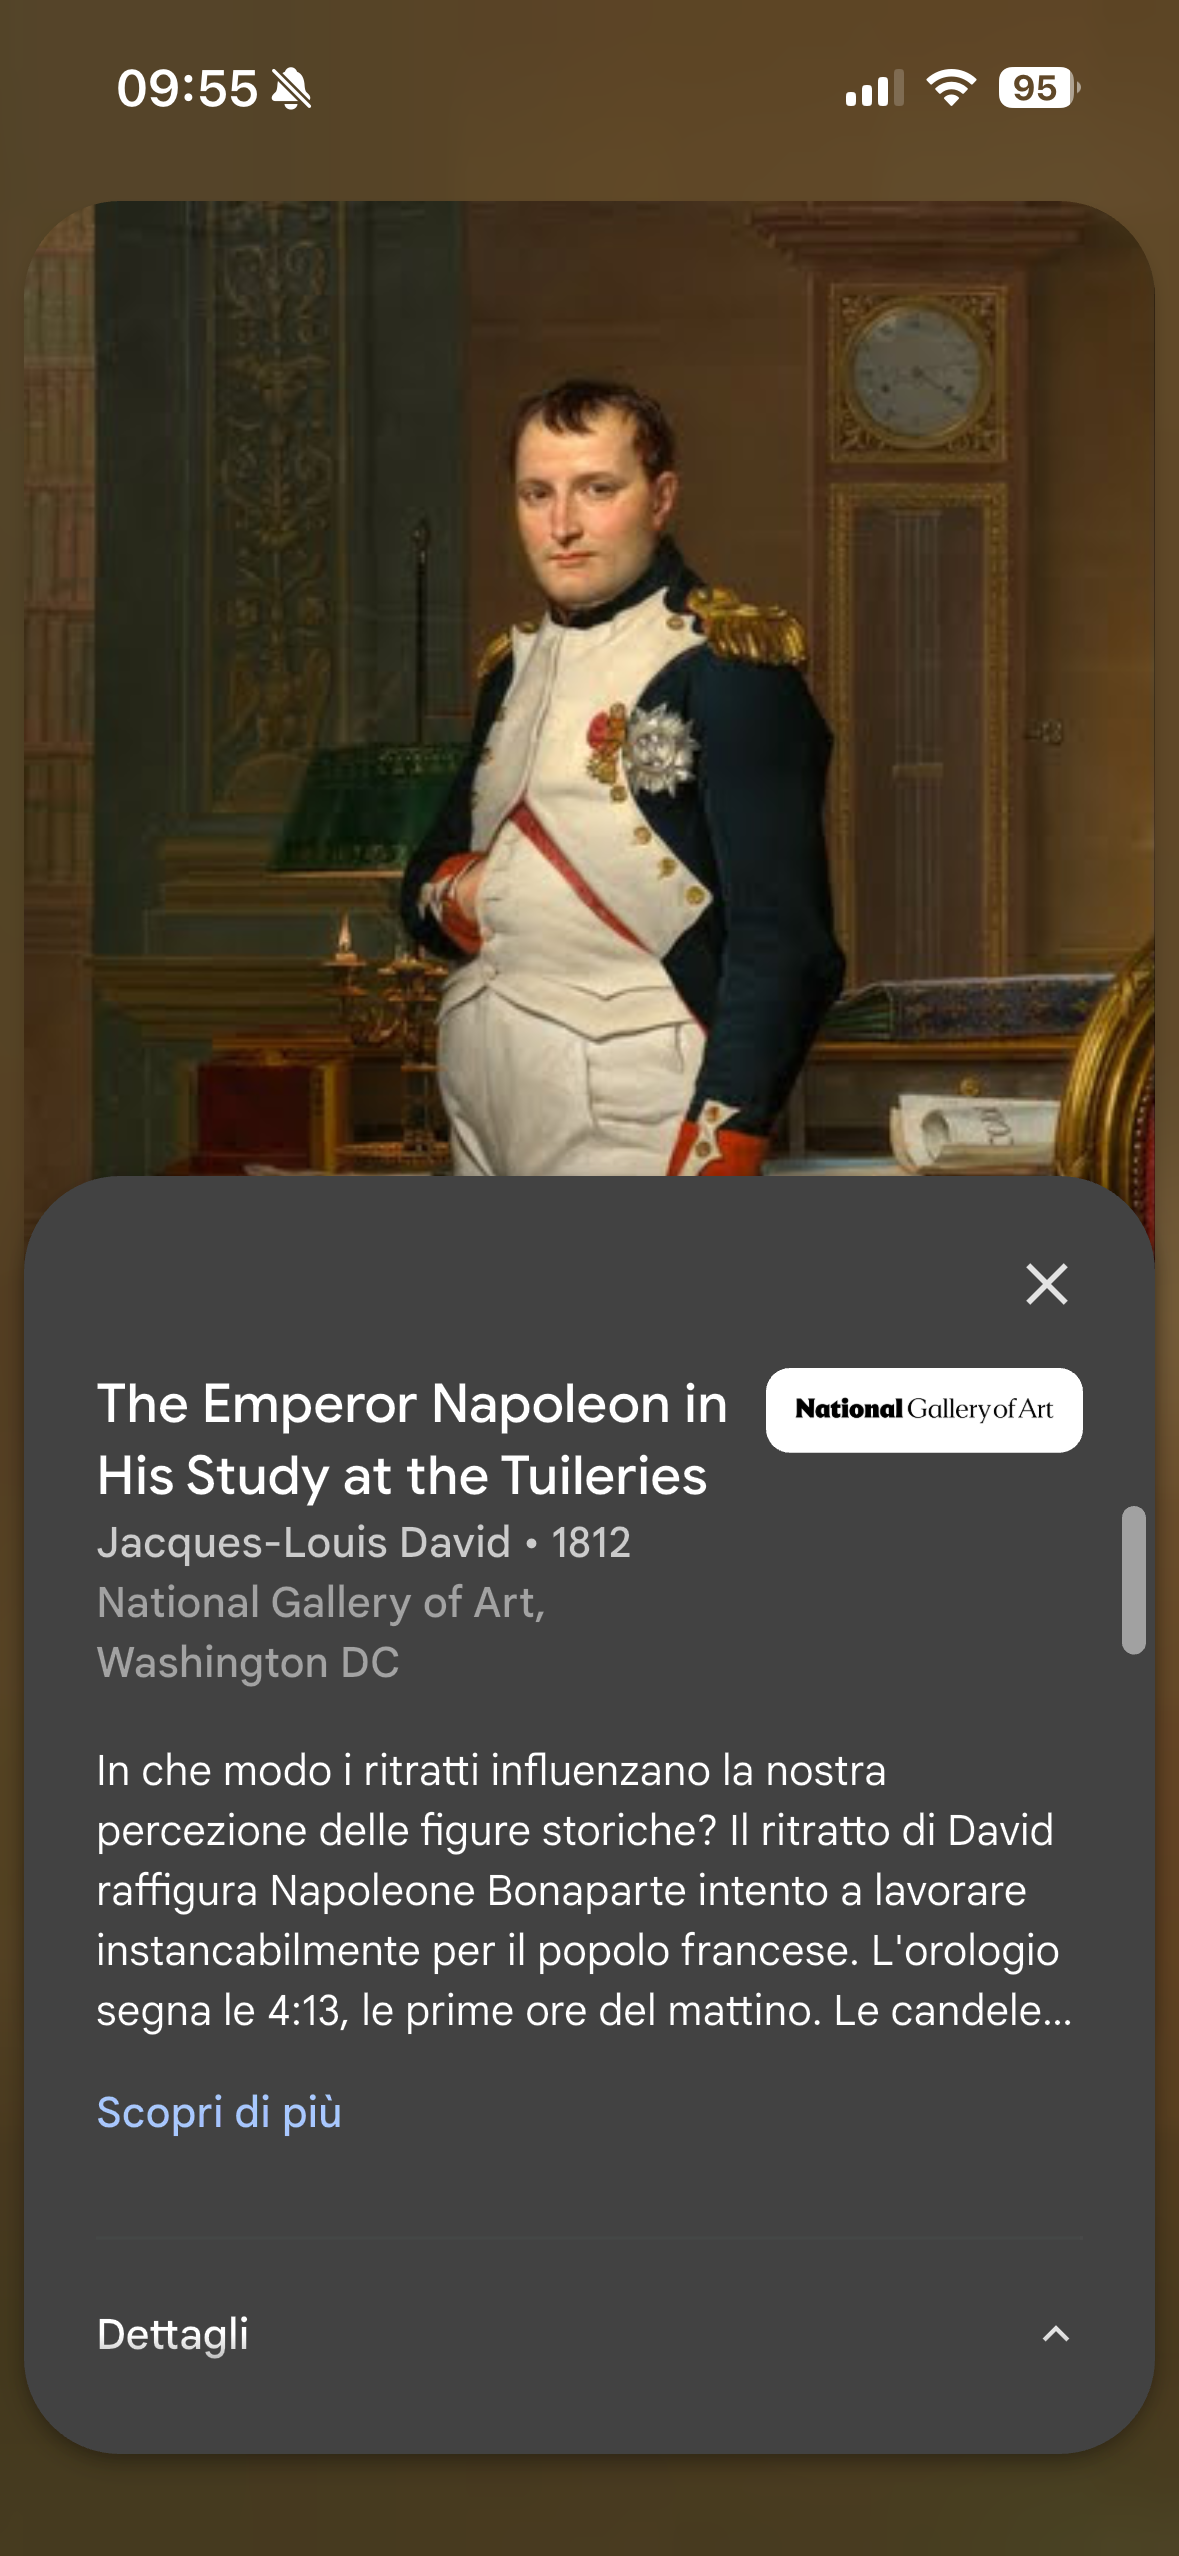
\includegraphics[width=\textwidth]{img/GA&C_02.PNG}
        \caption*{Modello 3D}
    \end{minipage}
    \hfill
    \begin{minipage}{0.31\textwidth}
        \centering
        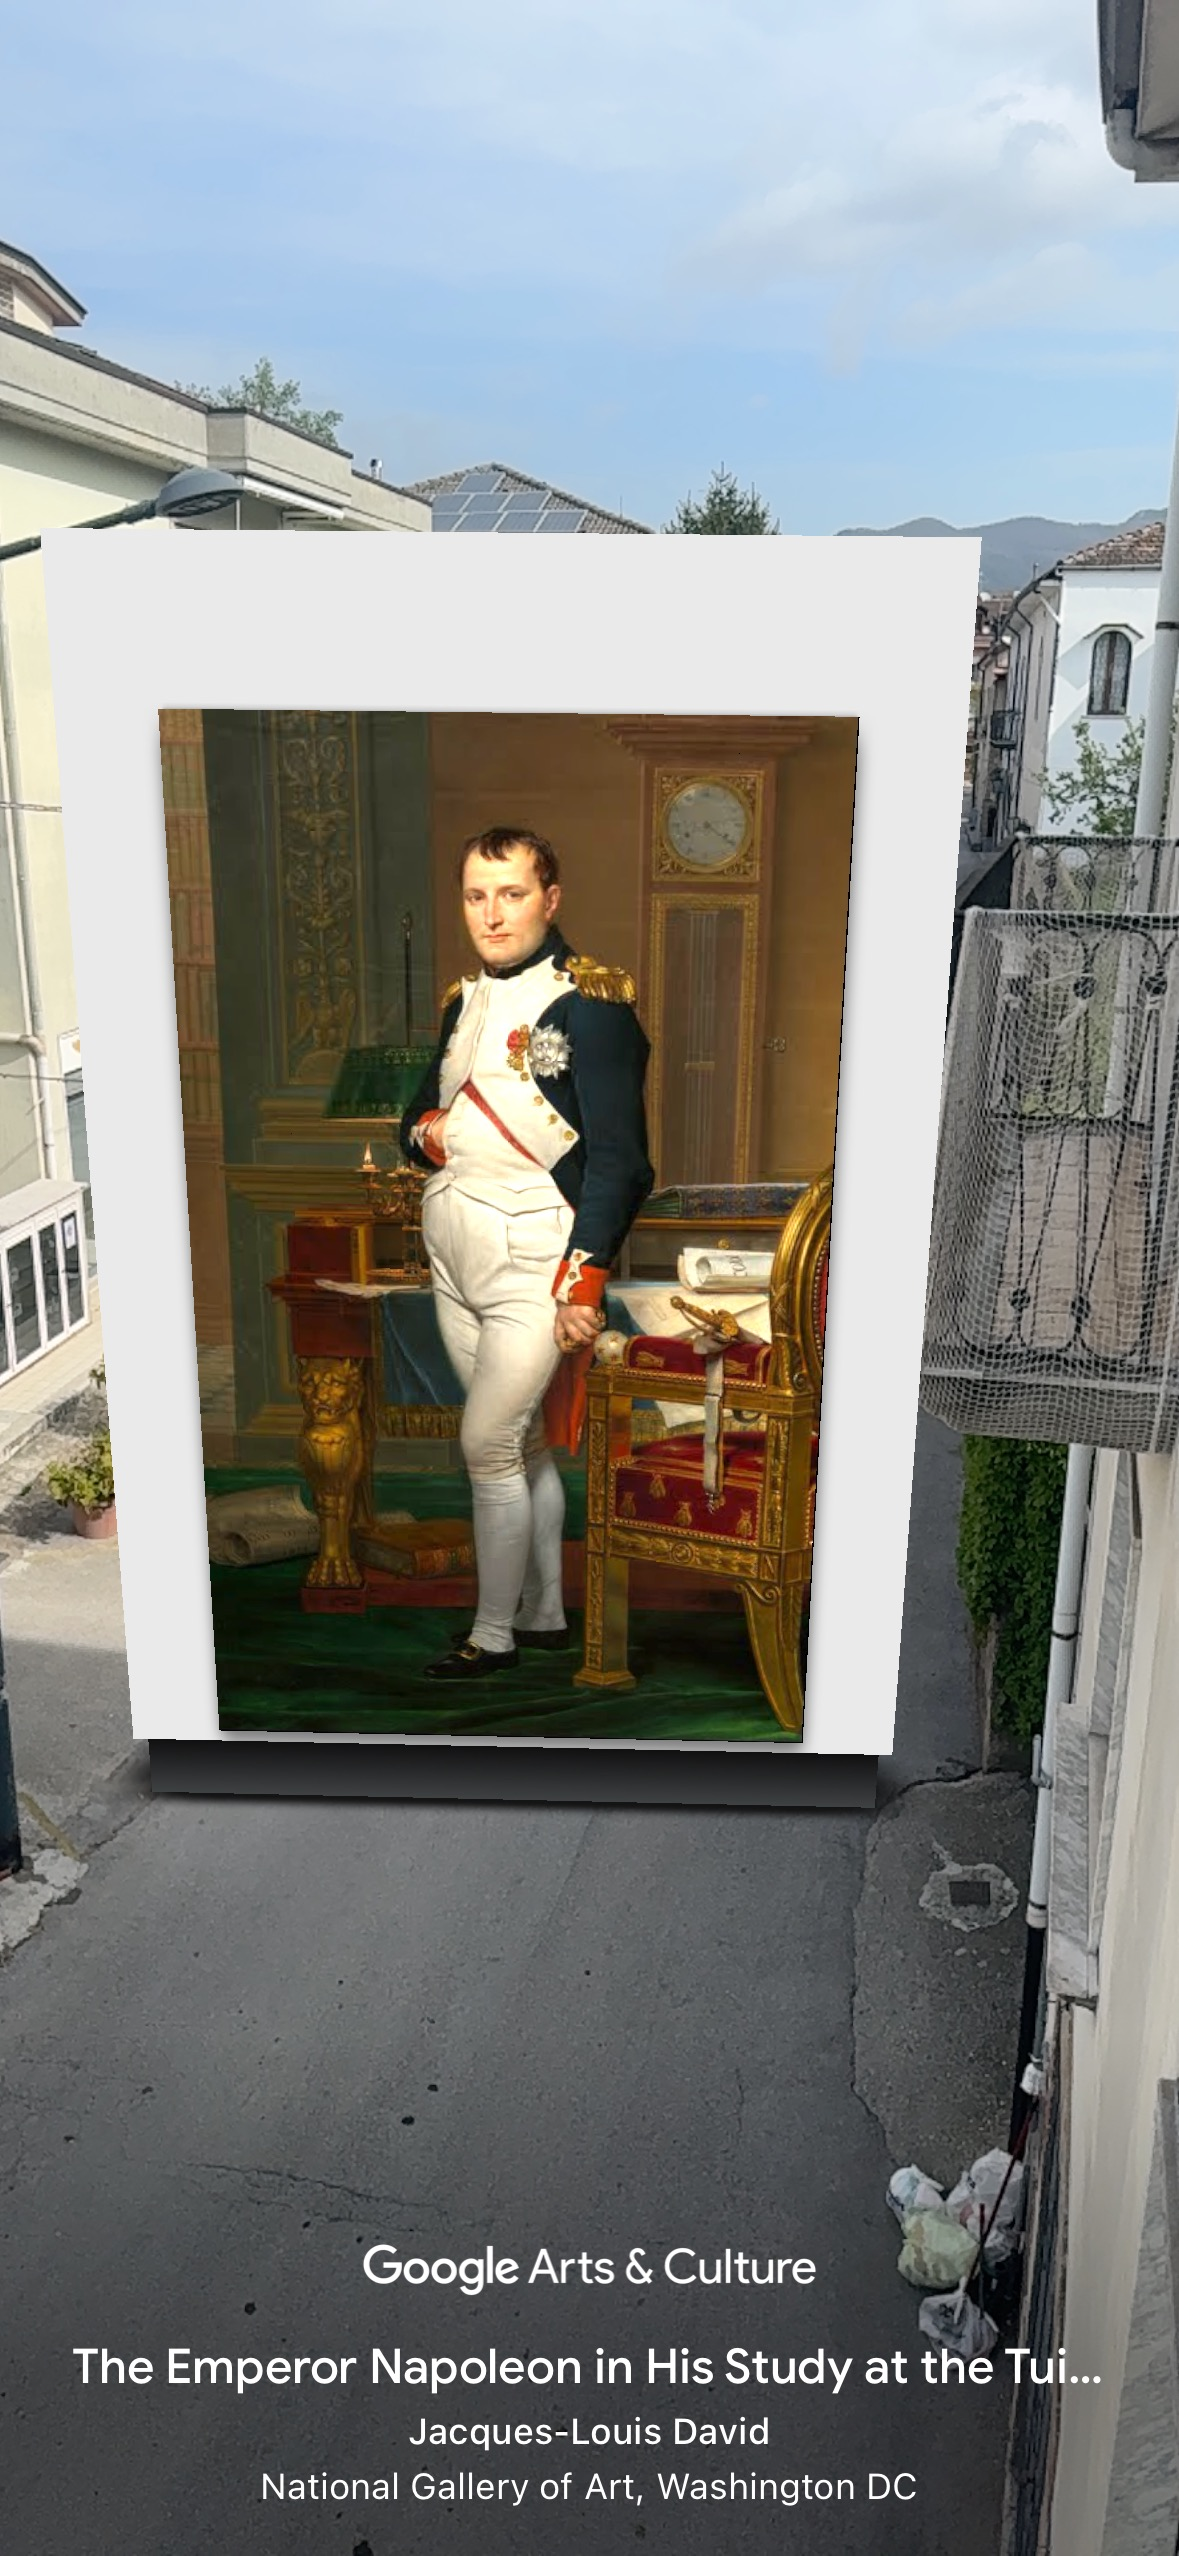
\includegraphics[width=\textwidth]{img/GA&C_03.JPG}
        \caption*{Interfaccia Home}
    \end{minipage}
\end{figure}

\subsubsection{Smartify}
Focalizzata sul riconoscimento istantaneo e sull'erogazione di contenuti audio, mostra limiti nella copertura di siti minori.
\nopagebreak
\begin{figure}[H]
    \centering
    \begin{minipage}{0.31\textwidth}
        \centering
        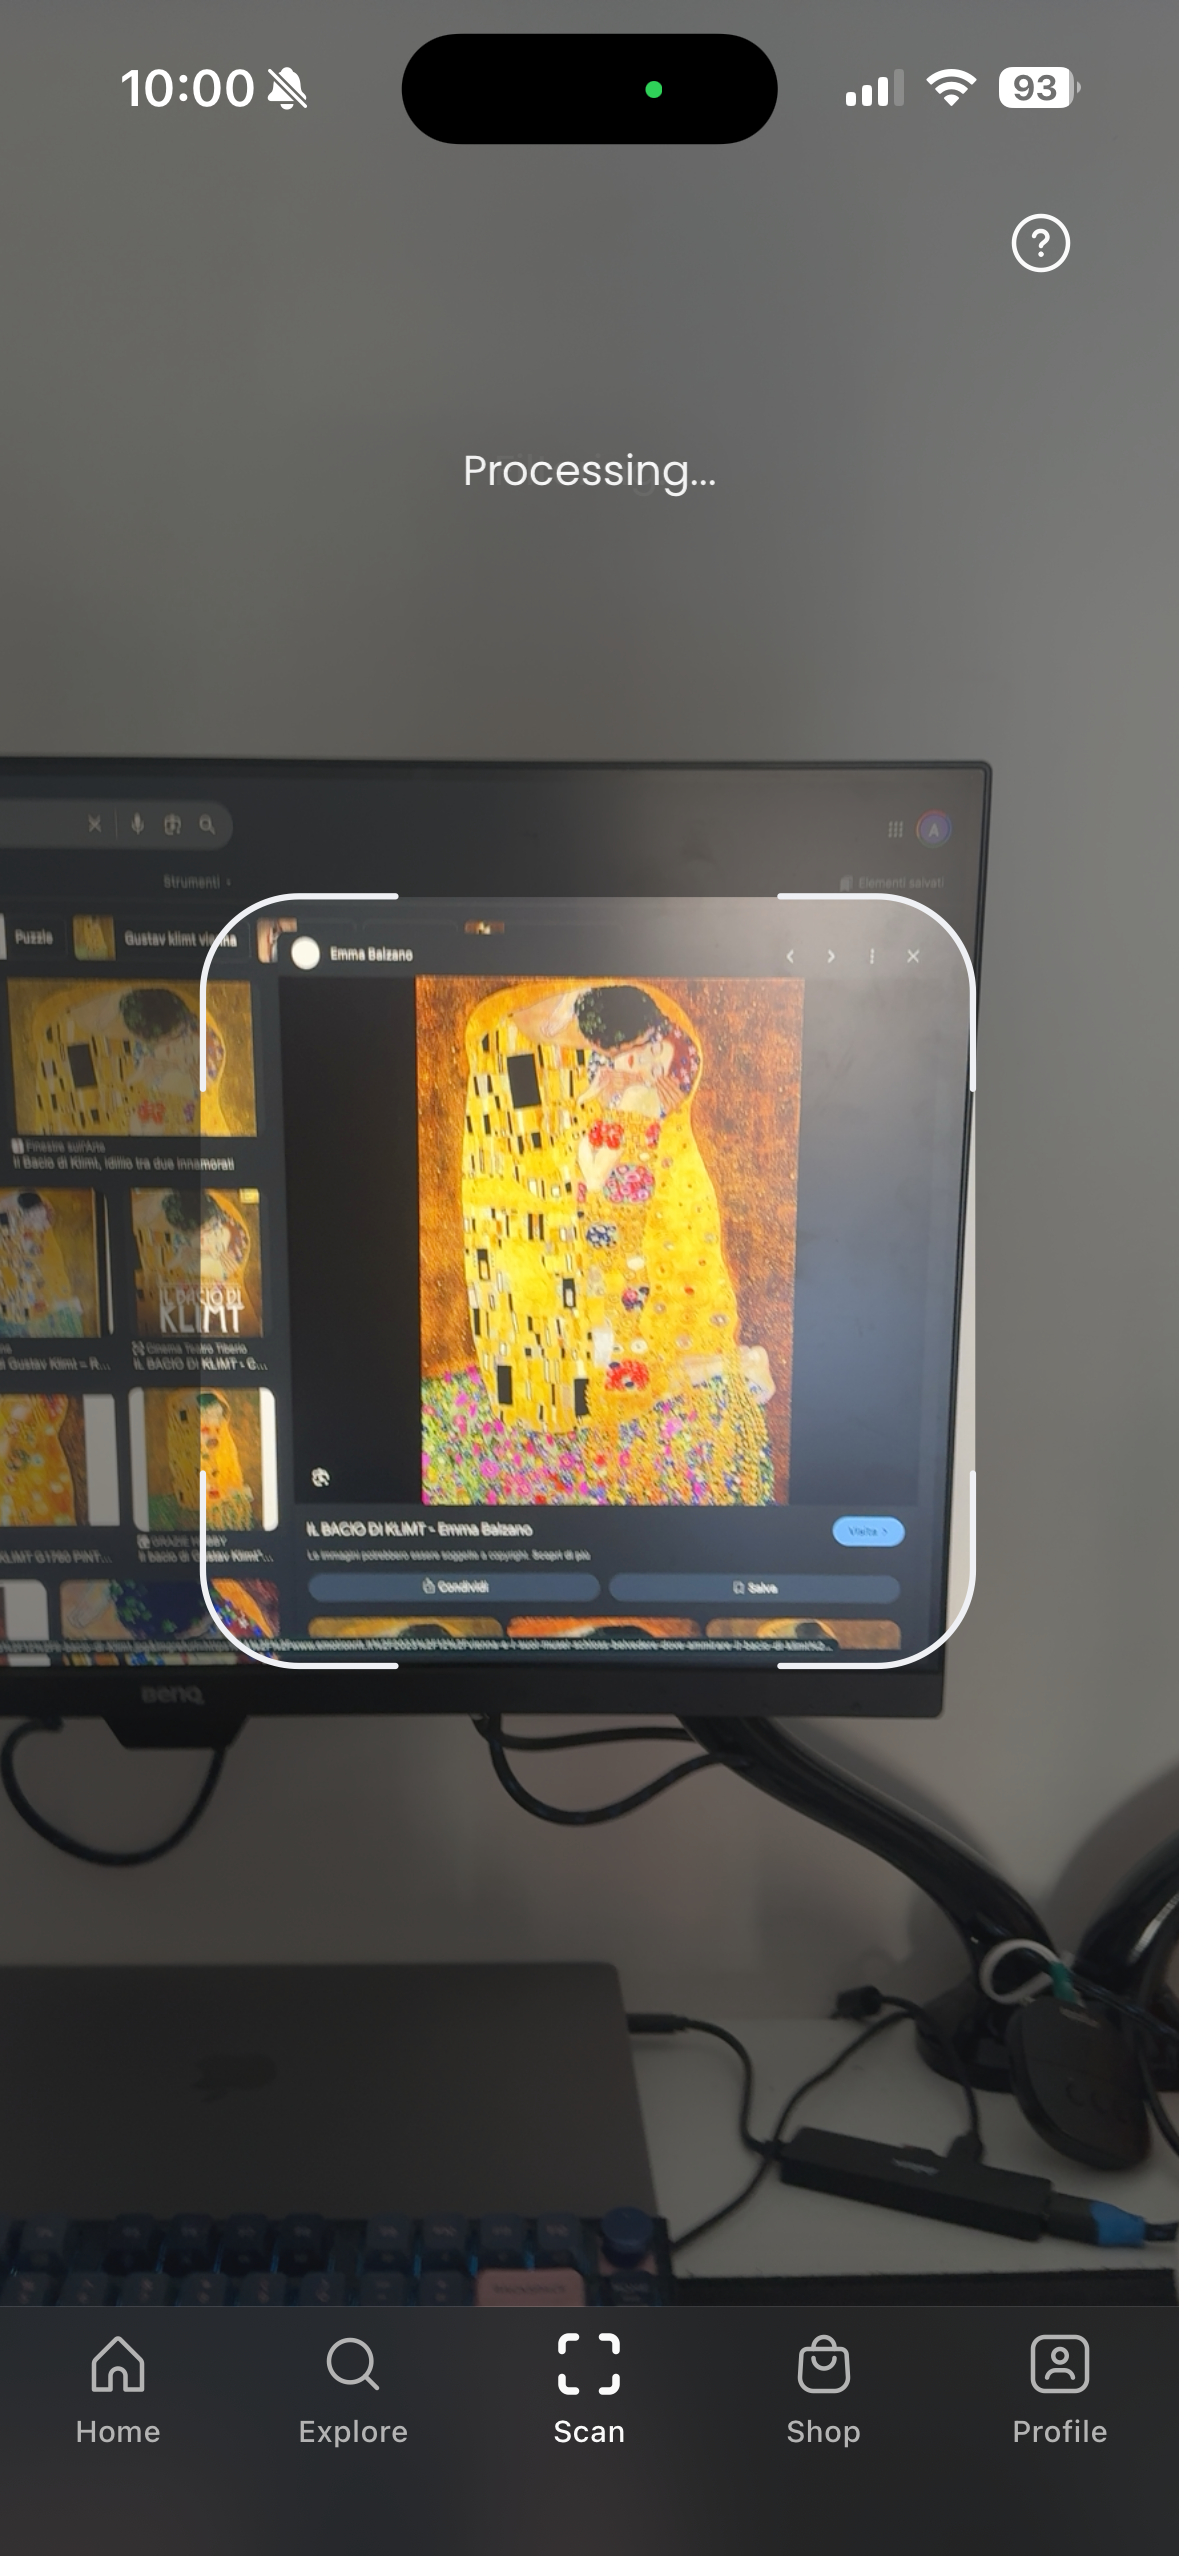
\includegraphics[width=\textwidth]{img/Smartify_01.PNG}
        \caption*{Riconoscimento}
    \end{minipage}
    \hfill
    \begin{minipage}{0.31\textwidth}
        \centering
        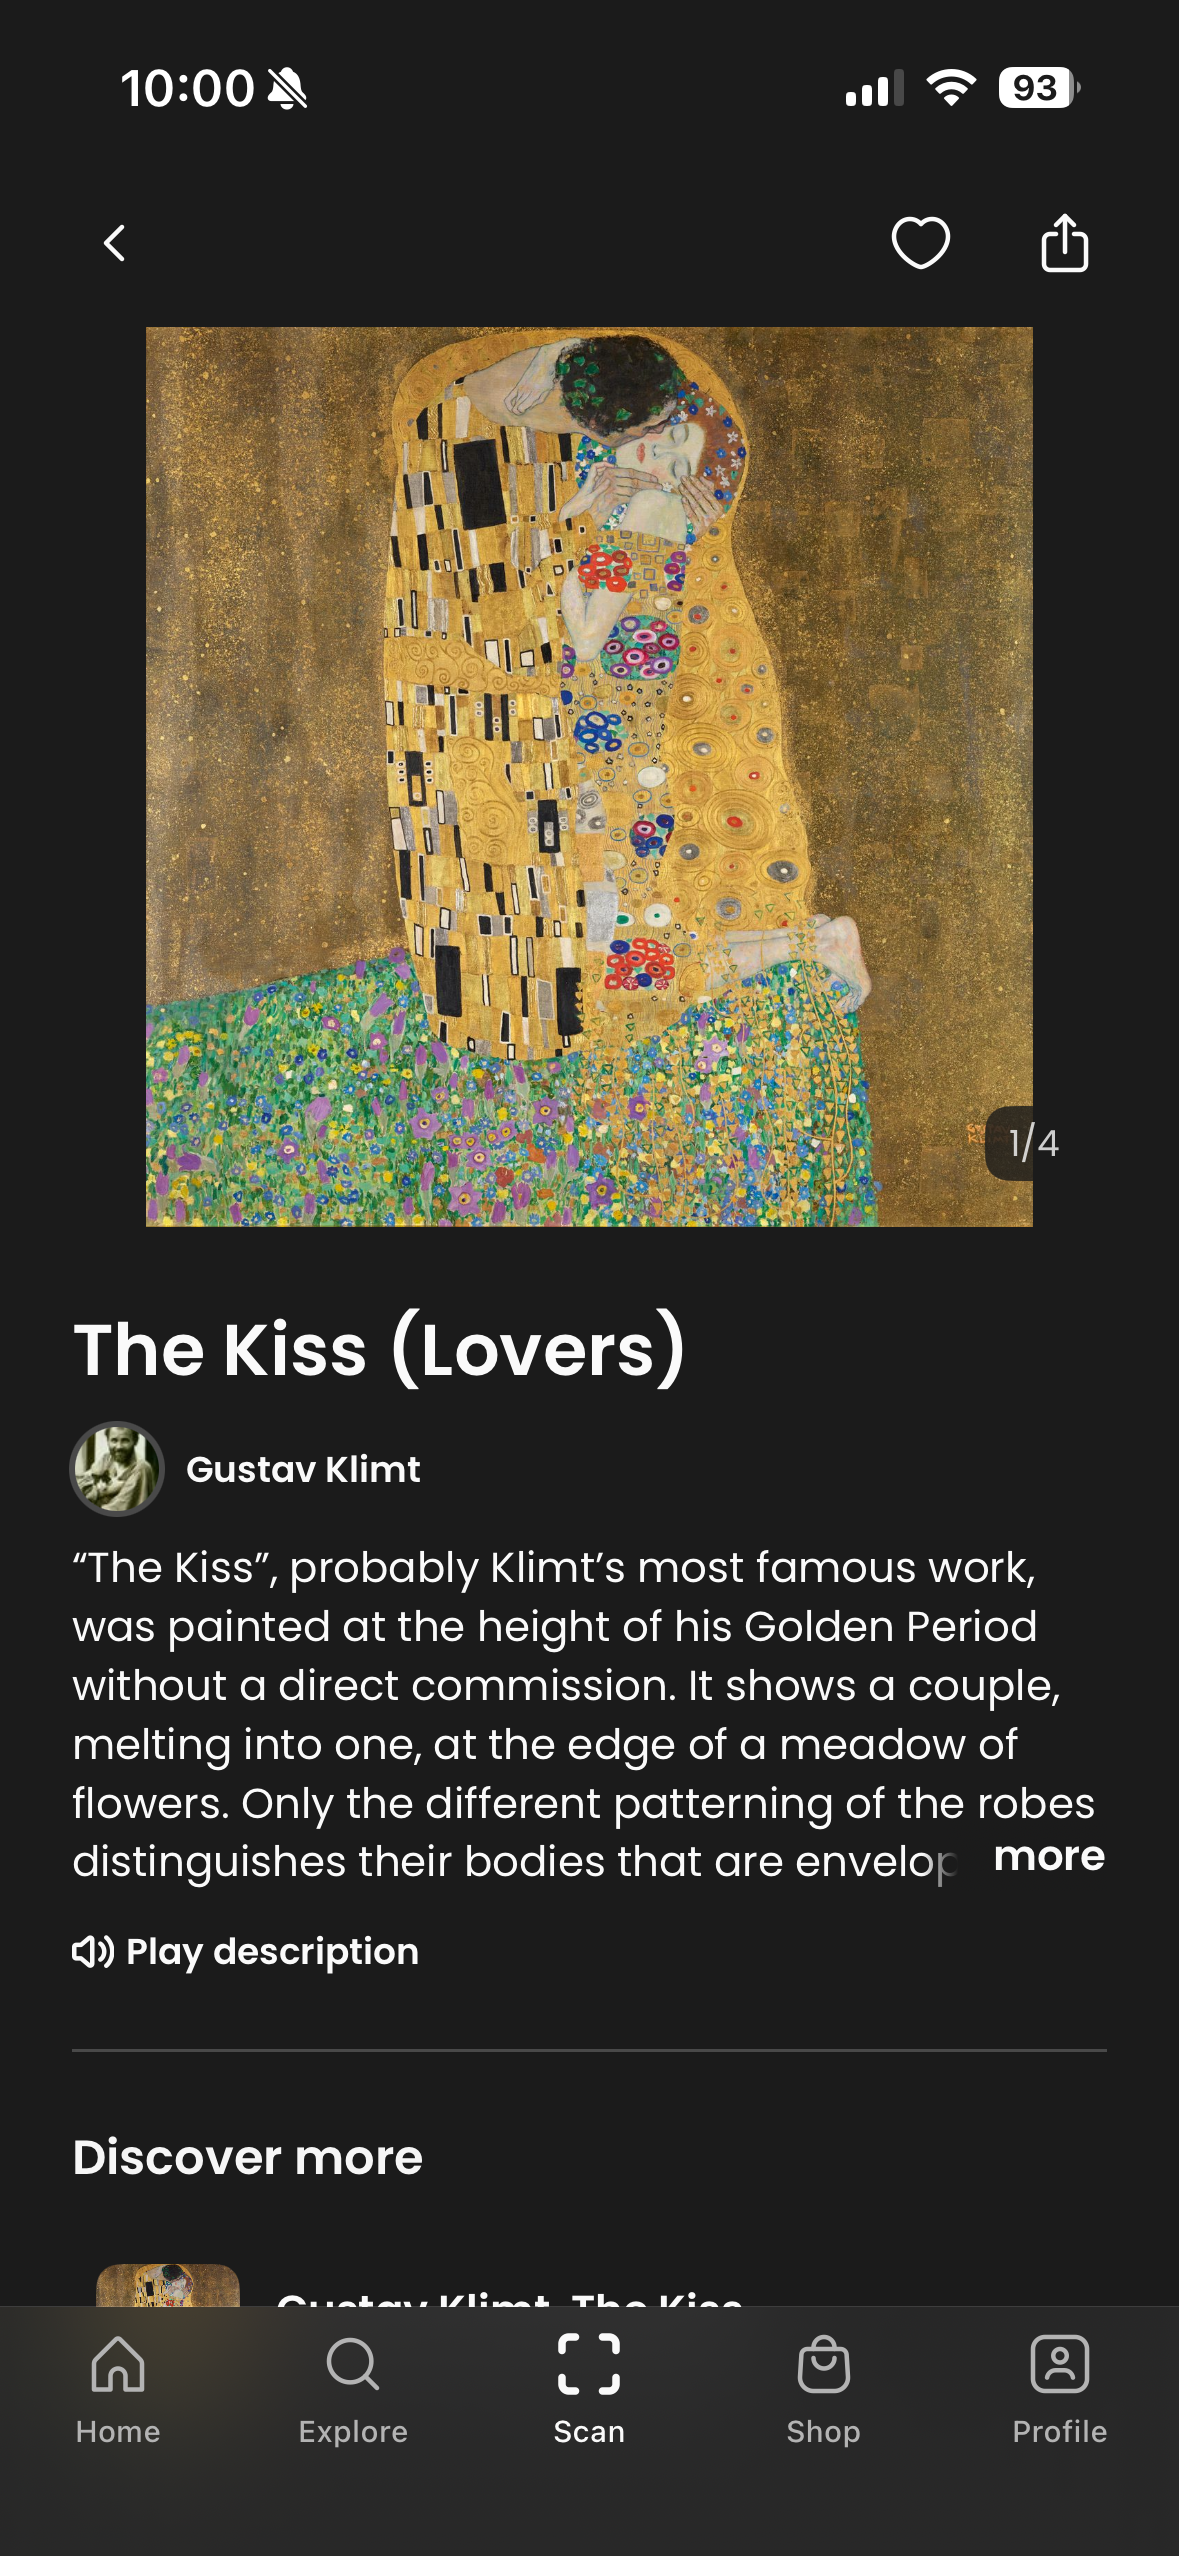
\includegraphics[width=\textwidth]{img/Smartify_02.PNG}
        \caption*{Dettagli Opera}
    \end{minipage}
    \hfill
    \begin{minipage}{0.31\textwidth}
        \centering
        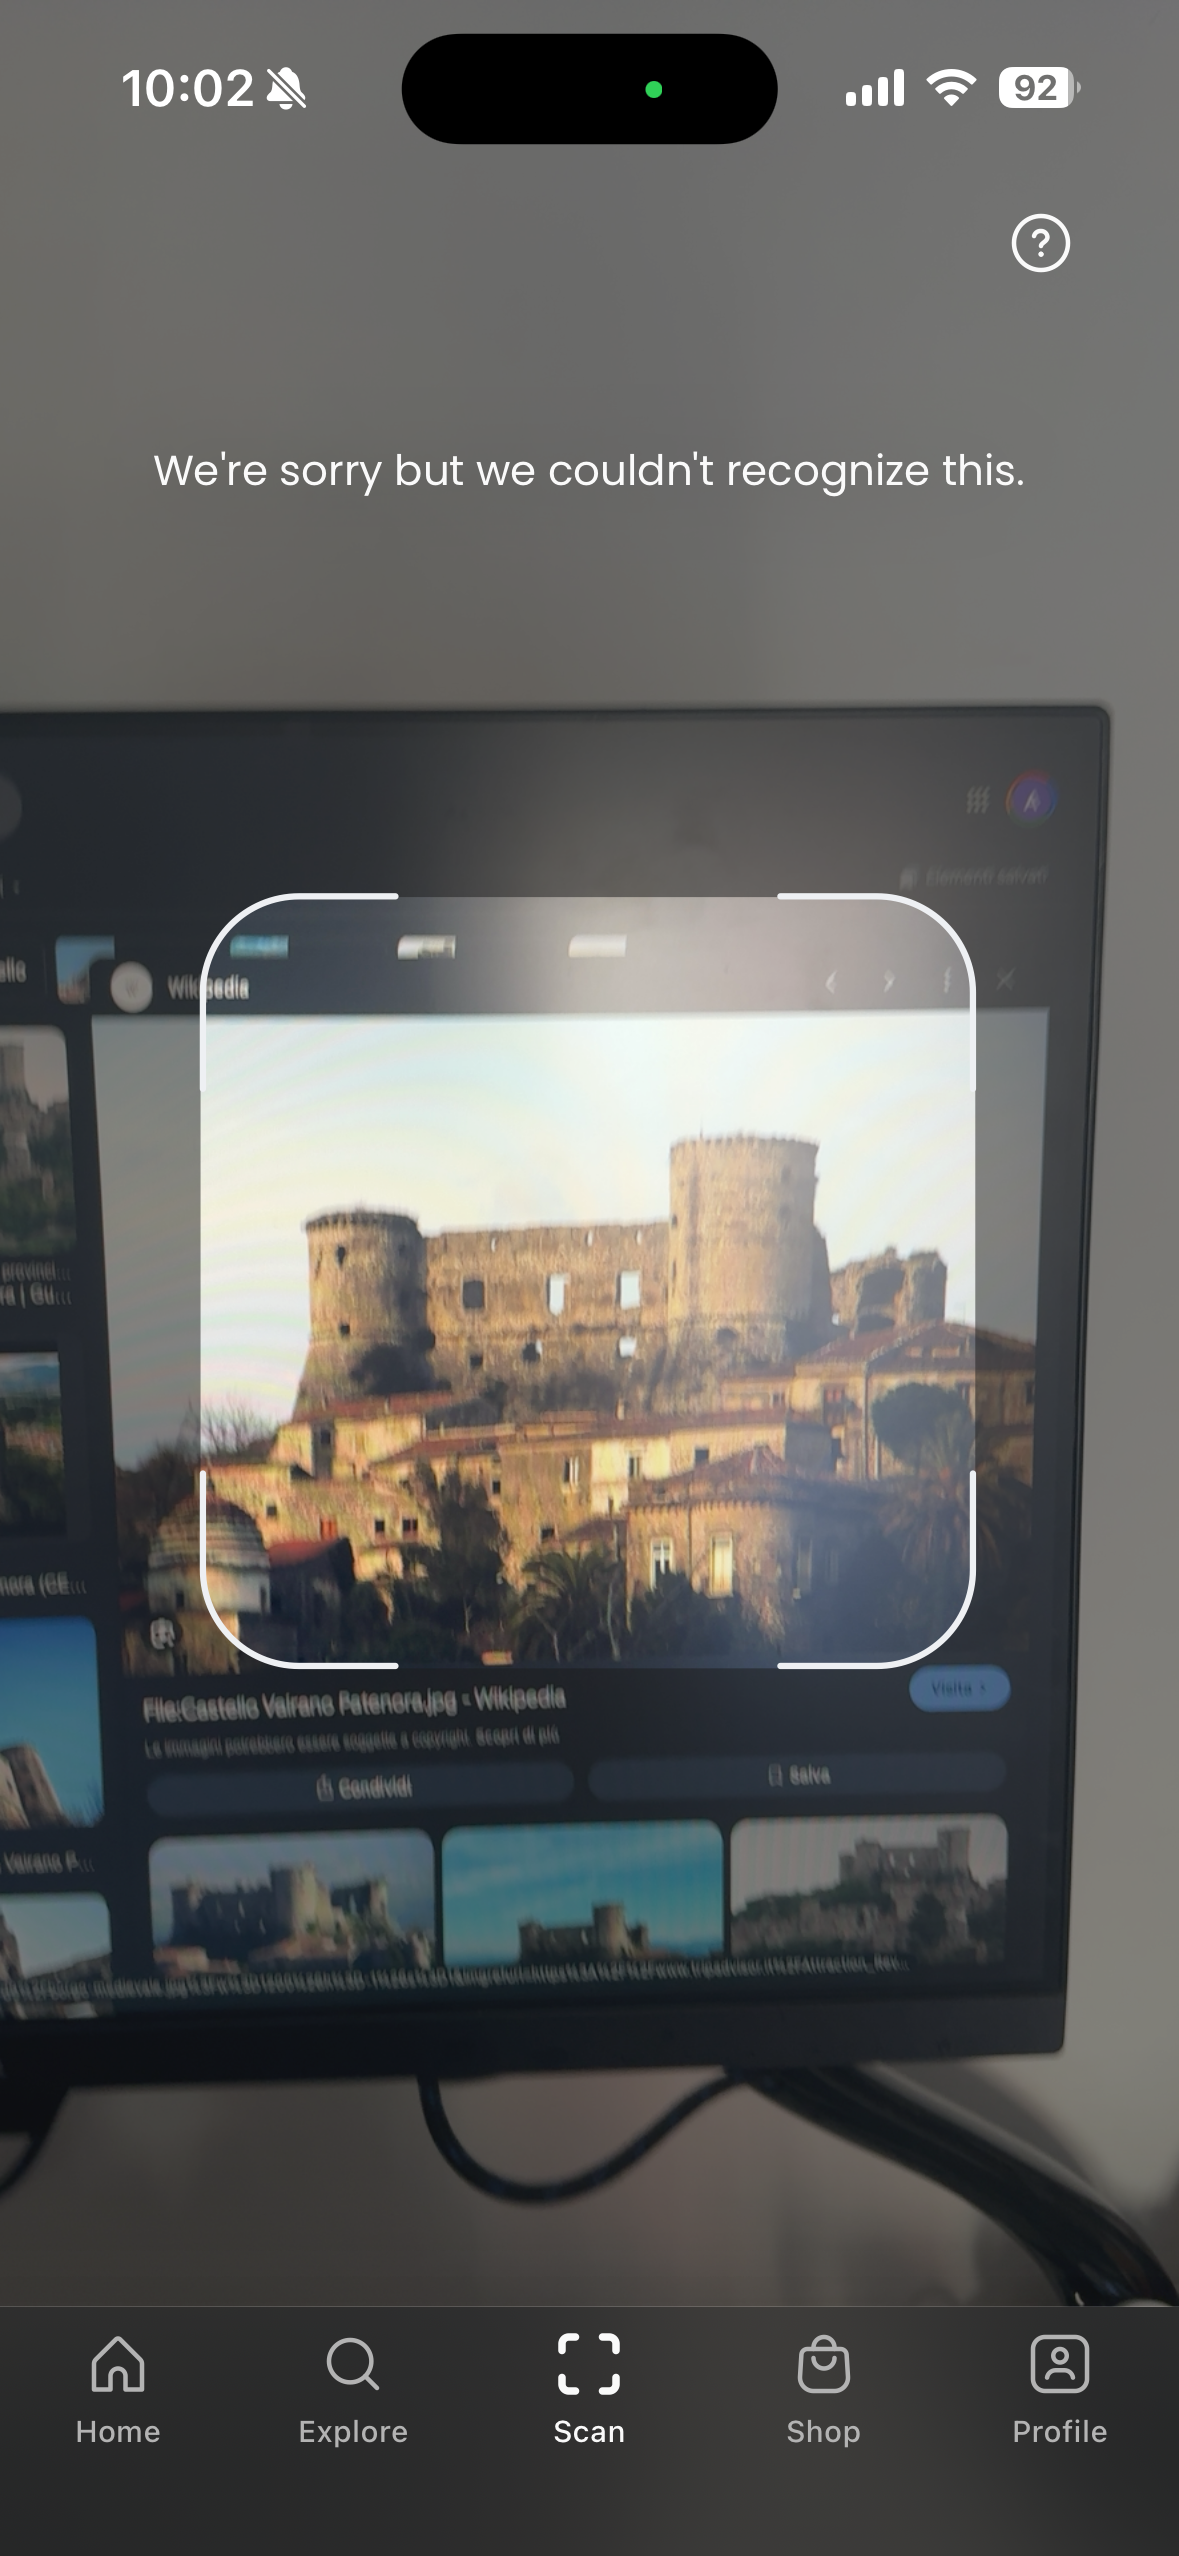
\includegraphics[width=\textwidth]{img/Smartify_03.PNG}
        \caption*{Mancato Riconoscimento}
    \end{minipage}
\end{figure}

\newpage
\subsubsection{Lazarillo}
Esempio di accessibilità funzionale pura, con interfaccia testuale ad alto contrasto e feedback audio per la navigazione. \textbf{Si evidenzia l'assenza di contenuti culturali.}
\nopagebreak
\begin{figure}[H]
    \centering
    \begin{minipage}{0.48\textwidth}
        \centering
        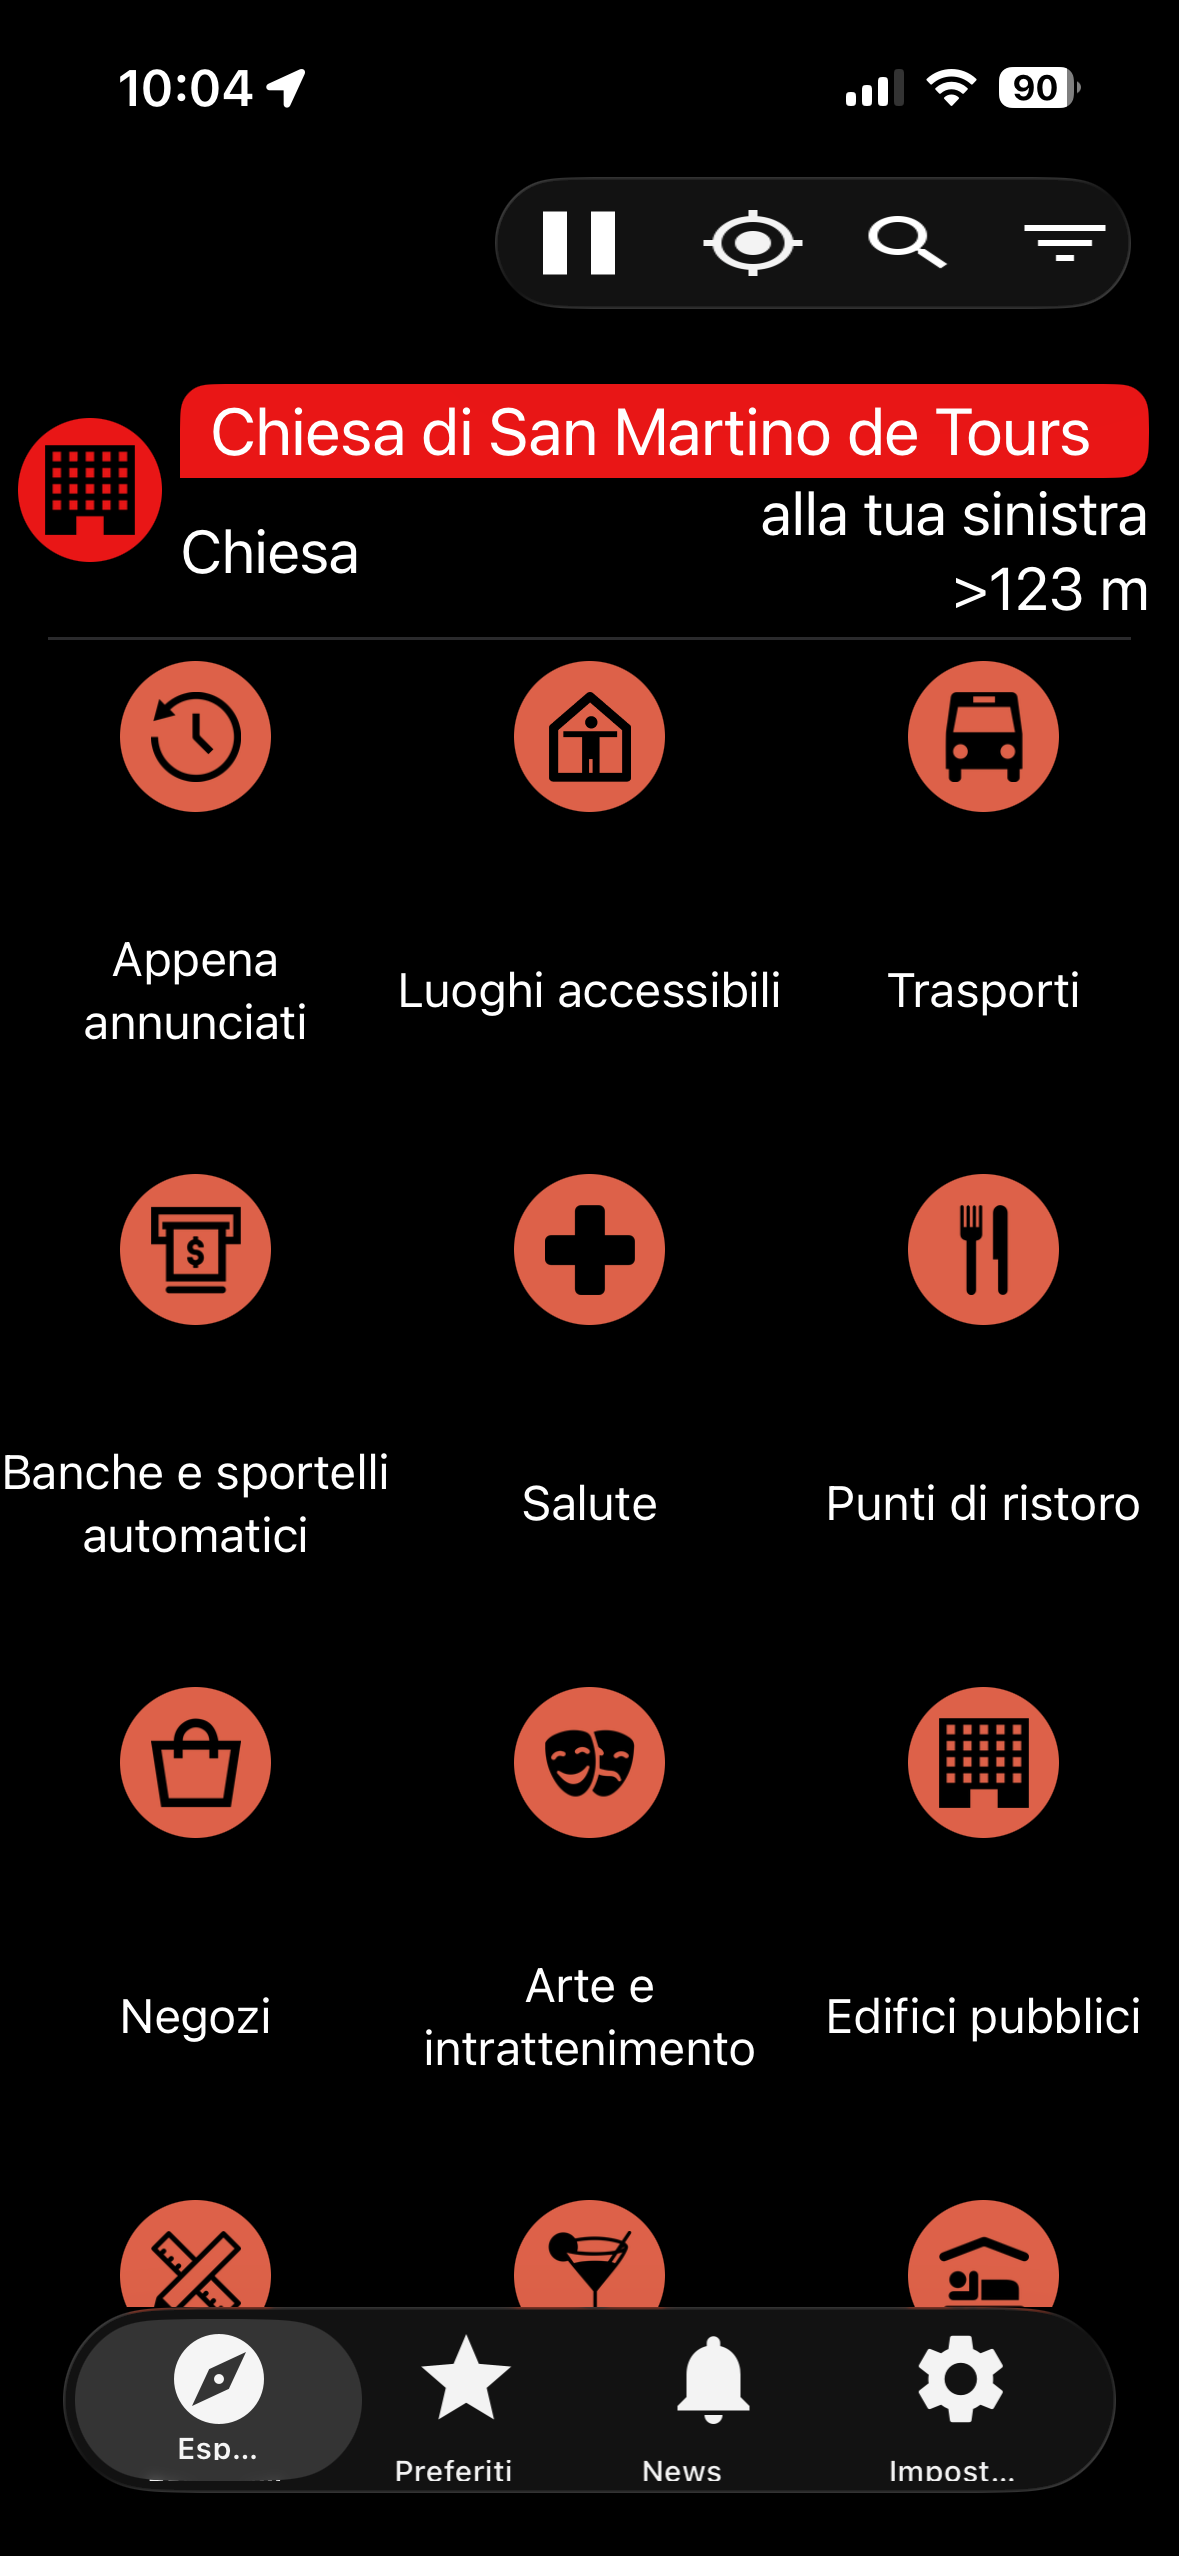
\includegraphics[width=\textwidth]{img/Lazarillo_01.PNG}
        \caption*{Esplorazione Luoghi}
    \end{minipage}
    \hfill
    \begin{minipage}{0.48\textwidth}
        \centering
        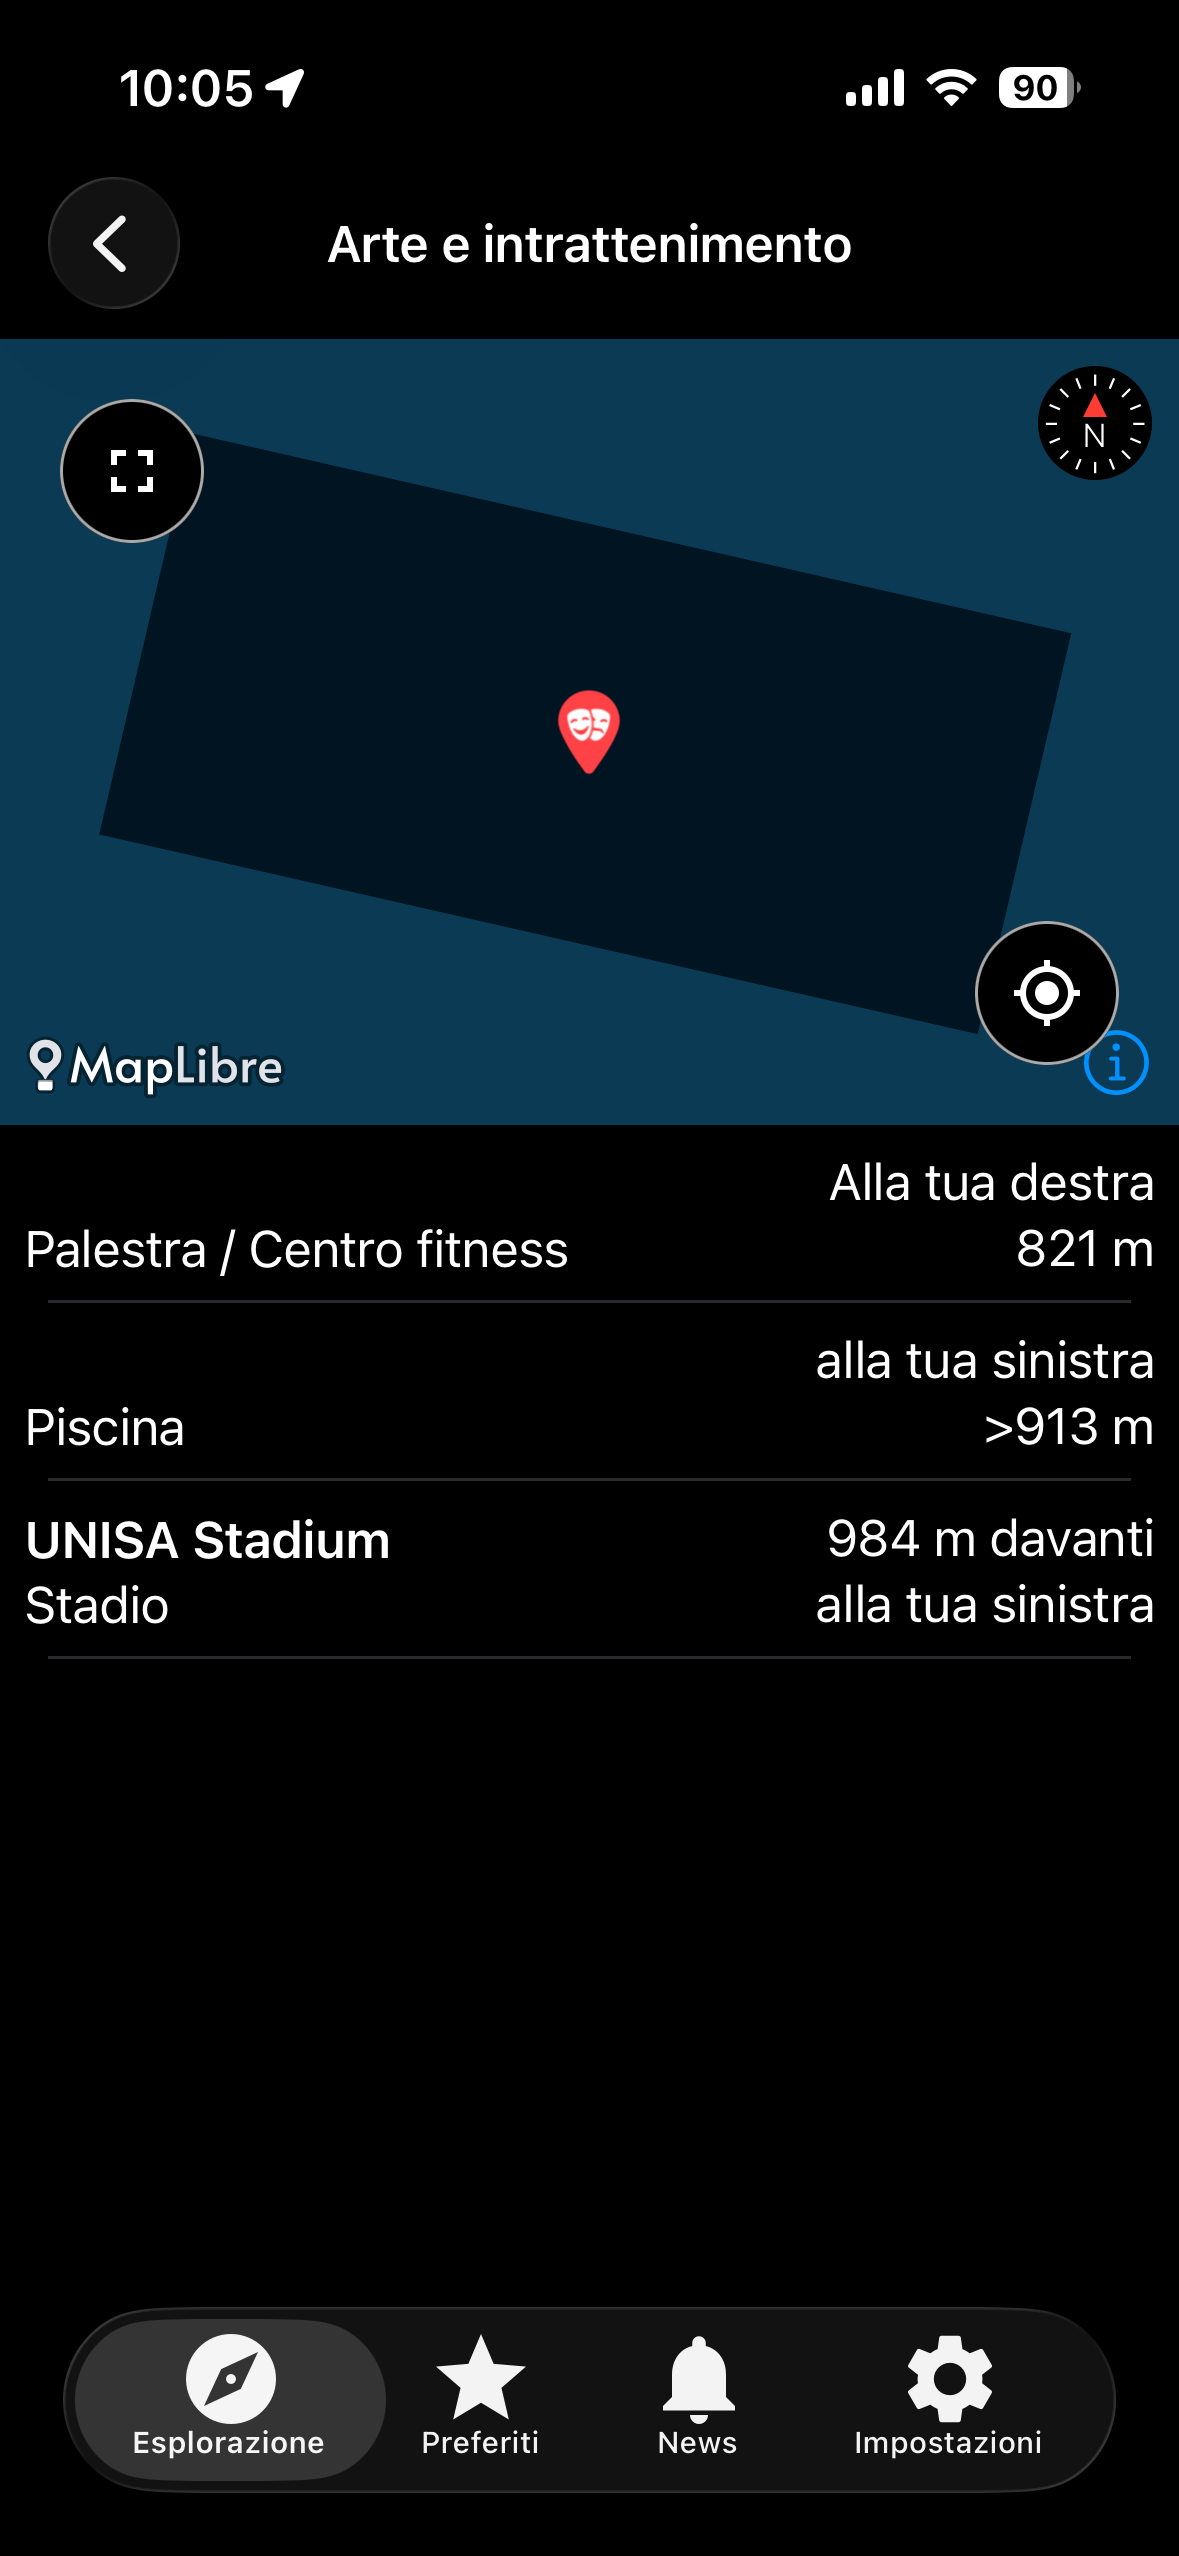
\includegraphics[width=\textwidth]{img/Lazarillo_02.PNG}
        \caption*{Navigazione Assistita}
    \end{minipage}
\end{figure}
